\documentclass[12pt,a4paper]{article}

% -------------------
% MARK: Packages
% -------------------

% import geometry package to update the document margins
\usepackage[margin=1in]{geometry}
% set the font to helvectica
\usepackage[scaled]{helvet}
\renewcommand\familydefault{\sfdefault}
% for type-setting
\usepackage{amsmath, amssymb, amsfonts, verbatim, pifont}
% for slashed out text
\usepackage[normalem]{ulem}
% for units and scientific notation
\usepackage[table]{xcolor}
\usepackage{siunitx}
% for references and URLs
\usepackage{hyperref, url}
% Natbib setup for author-year style
\usepackage{natbib}
 \bibpunct[, ]{(}{)}{,}{a}{}{,}%
 \def\bibfont{\small}%
 \def\bibsep{\smallskipamount}%
 \def\bibhang{24pt}%
 \def\newblock{\ }%
 \def\BIBand{and}%
% for graphics and figures
\usepackage{graphicx, subfig, tikz}
% force figures to stay in their sections
\usepackage[section]{placeins}
% for tables
\usepackage{booktabs, longtable, tabularx}
\usepackage{multicol, multirow}
\usepackage{adjustbox}
\usepackage[flushleft]{threeparttable}
% a package for working with .csv data for tables
\usepackage{csvsimple}
% setup the algorithm package
% ruled: show bars around title and bar at bottom
% lined: show the line column on the left of the algorithm
% linesnumbered: print line numbers for each line
\usepackage[ruled,lined,linesnumbered]{algorithm2e}
\DontPrintSemicolon % don't print the semicolon that \; usually prints
% fix overfull hbox errors from oddities like using
% quotes (``foo'') and etc.
\usepackage{microtype}

% -------------------
% MARK: Debugging Packages
% -------------------

% import a debugging package to show the margin boxes
% \usepackage{showframe}

% -------------------
% MARK: Declarations
% -------------------

% setup captions for tables and figures
\captionsetup[table]{%
  labelfont={bf},
  name={Table},
  labelsep=colon,
  justification=raggedright,
  singlelinecheck=false}
\captionsetup[figure]{%
  labelfont={bf},
  name={Figure},
  labelsep=colon,
  justification=raggedright,
  singlelinecheck=false}
\captionsetup[algorithm2e]{%
  labelfont={bf},
  name={Figure},
  labelsep=colon,
  justification=raggedright,
  singlelinecheck=false}

% set the graphics path to the img directory
\graphicspath{{img/}}

% -----------------------------------------------------------------------------
% MARK: algorithm2e stuff
% -----------------------------------------------------------------------------

% params
% \SetKwInOut{Objects}{$\CKmatrix{O}$}
% \SetKwInOut{Weights}{$\CKvector{w}$}

% -------------------
% MARK: Headers
% -------------------

% headers and footers
\usepackage{fancyhdr}
\setlength{\headheight}{15pt}
\pagestyle{fancy}
\lhead{KautenjaDSP}
\rhead{\itshape 106 v1.3.4}
\cfoot{\thepage}

% start the document
\begin{document}

% -------------------
% MARK: Title Page
% -------------------

% fancyhdr directive to remove headers from this title page
\thispagestyle{empty}
% center the title page contents
\vspace*{\fill}
\begin{center}

\includegraphics{106-Logo}
\linebreak\linebreak\linebreak\linebreak
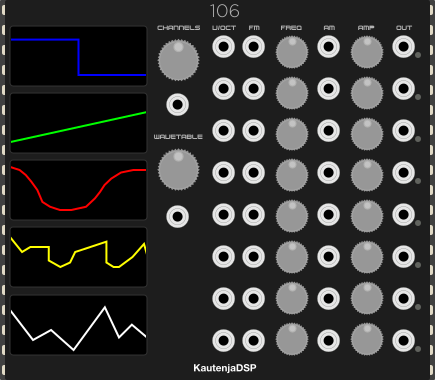
\includegraphics{106-Module}
\linebreak\linebreak\linebreak\linebreak

\includegraphics{KautenjaDSP}
\end{center}
\vspace*{\fill}
\clearpage

% -------------------
% MARK: Overview
% -------------------

\section{Overview}

106 is an emulation of the Namco 106 audio processing unit from the Nintendo Entertainment System (NES) for VCV Rack. The Namco 106 chip contains eight channels of wave-table synthesis and 128 bytes of operational RAM. The wave-tables are 4-bit and can be as long as 63 samples. This module uses a bank of five 32-sample wave-tables to act as the waveform for all eight channels.

Namco 106 provides the key features of the Namco 106 chip, namely,
\begin{itemize}
  \item \textbf{Wave-table synthesis:} 8 channels of wave-table synthesis with bit depth of 4 bits and table size of 32 samples
  \item \textbf{Waveform morph:} 5 banks of wave-tables to morph between using 32-bit floating point linear interpolation (not very retro, but it sounds nice)
  \item \textbf{Frequency control:} 18-bit frequency control with linear frequency modulation
  \item \textbf{Amplitude modulation:} 4-bit amplifier with linear amplitude modulation
  \item \textbf{Namco 106 compute limitation:} activating each additional channel (up to 8) reduces the amount of compute available for all channels. This causes all channels to drop in frequency when additional channels are activated.
\end{itemize}

% -------------------
% MARK: Panel Layout
% -------------------

\section{Panel Layout}

\begin{center}
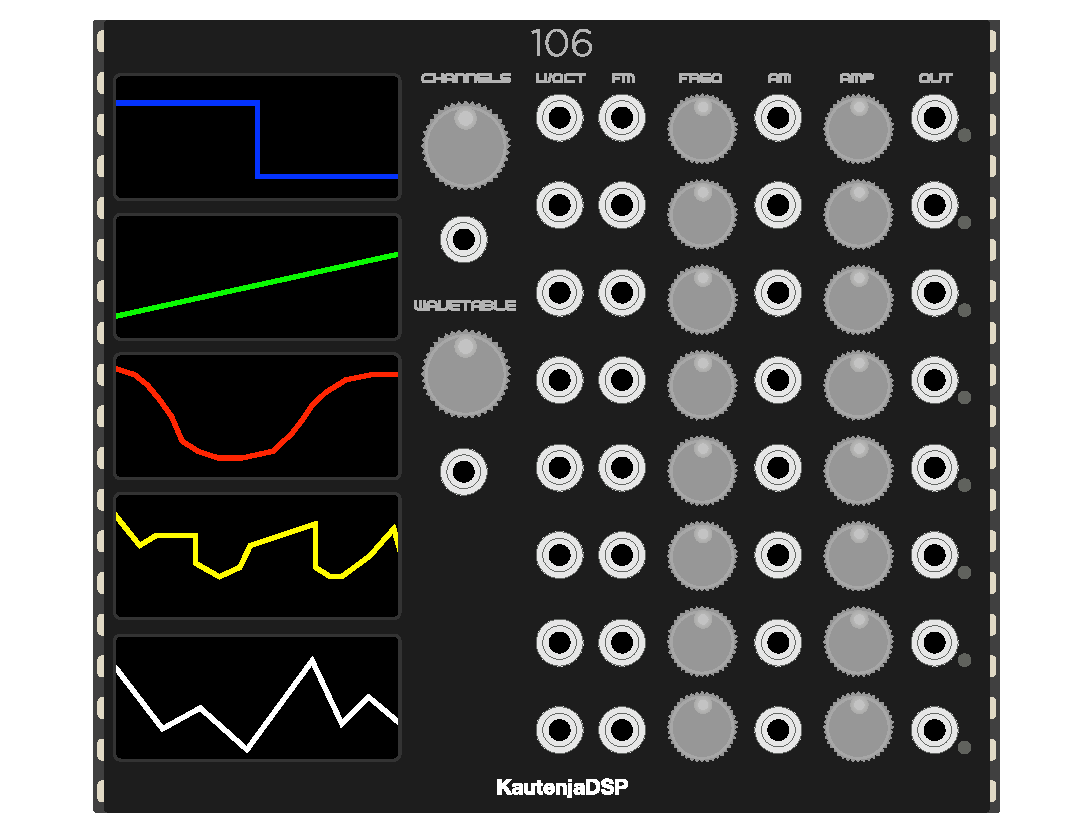
\includegraphics{106-Manual}
\end{center}

\begin{enumerate}
  \item Waveform selection. Draw arbitrary waveforms using the mouse pointer.
  \item Channel selection. The big knob determine the number of channels in use by the chip. The small knob acts as an attenuverter for the linear CV input.
  \item Wave-table selection. The big knob determine the wave-table used by the chip. The small knob acts as an attenuverter for the linear CV input. Wave-table morphing is accomplished through 32-bit floating point linear interpolation.
  \item $V$/Octave inputs for the eight channels.
  \item CV linear frequency modulation for the eight channels.
  \item Coarse frequency control over the eight channels.
  \item CV linear amplitude modulation for the eight channels using the 4-bit amplifier.
  \item Coarse amplitude control over the eight channels using the 4-bit amplifier.
  \item Channel outputs for the eight channels, ${\approx}10V_{pp}$. The LED indicates whether the channel is activated based on (2).
\end{enumerate}

% -------------------
% MARK: References
% -------------------

\clearpage
\renewcommand\refname{References \& Acknowledgments}
\nocite{*}
\bibliographystyle{apalike}
\bibliography{references}

\end{document}
